\section{Integração Numérica em um Domínio Bidimensional}

\begin{figure}[htb]
 \centering
 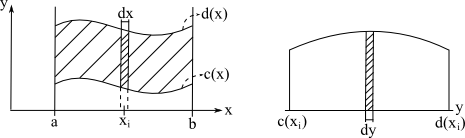
\includegraphics[scale=1.0]{capitulos/capitulo2/figuras/int_num_dom_bid1.png}
 \caption{Integração Numérica em um Domínio Bidimensional}
 \label{fig:int_num_dom_bid1}
\end{figure}

\begin{equation}
 \label{cap2:sec9:eq1}
 I = \int_a^b \left[ \int_{c\,(x)}^{d\,(x)} \, f\,(x,\,y) \, dy \right] \, dx
\end{equation}

\begin{equation}
 \label{cap2:sec9:eq2}
 G\,(x) = \int_{c\,(x)}^{d\,(x)} \, f\,(x,\,y) \, dy
\end{equation}

\begin{equation}
 \label{cap2:sec9:eq3}
 I = \int_a^b \, G\,(x) \, dx
\end{equation}

\begin{equation}
 \label{cap2:sec9:eq4}
 I = \sum_{i = 0}^N \, w_i \, G\,(x_i)
\end{equation}

\begin{equation}
 \label{cap2:sec9:eq5}
 G\,(x_i) = \sum_{j = 0}^M \, w_j \, f\,(x_i,\,y_j)
\end{equation}

\begin{example}
 Calcule a integral dupla

\[
 I = \int_a^b \left[ \int_{c\,(x)}^{d\,(x)} \, sin\,(x+y) \, dy \right] \, dx
\]

pela regra $\displaystyle \frac{1}{3}$ de Simpson.

\[
 \begin{array}{l}
  a = 1 \\
  b = 3 \\
  c\,(x) = ln\,(x) \\
  d\,(x) = 3 + e^{x/5}
 \end{array}
\]

\textbf{Solução:}

\begin{figure}[htb]
 \centering
 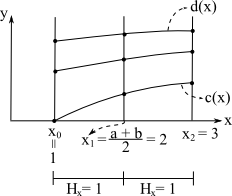
\includegraphics[scale=1.0]{capitulos/capitulo2/figuras/int_num_dom_bid2.png}
 \caption{?}
 \label{fig:int_num_dom_bid2}
\end{figure}

\[
 \begin{array}{ll}
  I & = \displaystyle \frac{H_x}{3} \, \left[ G\,(x_0) + 4\,G\,(x_1) + G\,(x_2) \right] \vspace*{0.2cm} \\
    & \approx \displaystyle \frac{H_x}{3} \left[ \int_{ln\,(1)}^{3+e^{(1/5)}} sin\,(1+y)\,dy \, + \, 4\,\int_{ln\,(2)}^{3+e^{(2/5)}} sin\,(2+y)\,dy \, + \, \int_{ln\,(3)}^{3+e^{(3/5)}} sin\,(3+y)\,dy \right] \\
    & \approx \displaystyle \frac{1}{3} \left[ \int_0^{4.2214} sin\,(1+y)\,dy \, + \, 4\,\int_{0.6931}^{4.4918} sin\,(2+y)\,dy \, + \, \int_{1.0986}^{4.8221} sin\,(3+y)\,dy \right]
 \end{array}
\]

\[
 \begin{array}{ll}
  G\,(x_0) & \approx \displaystyle \frac{2.11070}{3} \, \left[ sin\,(1+0) + 4\,sin\,(1+2.11070) + sin\,(1+4.2214) \right] \\
           & = 0.064581 \\
  G\,(x_1) & \approx \displaystyle \frac{1.89935}{3} \, \left[ sin\,(2+0.6931) + 4\,sin\,(2+2.59245) + sin\,(2+4.4918) \right] \\
           & = -2.1086 \\
  G\,(x_2) & \approx \displaystyle \frac{1.86175}{3} \, \left[ sin\,(3+1.0986) + 4\,sin\,(3+2.96035) + sin\,(3+4.8221) \right] \\
           & = -0.67454
 \end{array}
\]

\[
 I \approx \frac{1}{3} \, \left[ 0.064581 + (4)\,(-2.1086) - 0.67454 \right] = -3.0148
\]

\end{example}